July 2nd, 2004, shortly after midnight.

\begin{quotation}
My emotions are gaining distinct colors, like a kind of twisted synaesthesia.  There's definitely a sense of physical location associated with each emotion, and it's not always internal.  There may also be a tactile part to this, but I have yet to experience it in any different places or with any different touches, so it may just be one continuous headache that goes latent occasionally.

An example: when pondering ****, a luminescent fuschia color that seems to be flowing in the right hemisphere of my brain; when thinking of ******* and snuggling, a warm, earthy brown with a little bit of green in a pine-needle-ish pattern about a foot and a half in front of me and slightly to the left; tiredness is off-white everywhere and blind hopelessness is bright blue wrapped around my mind.  The headache moves around, but it's mostly at the lower, back, right side of my head.  Ibuprofin works well.

This isn't what I meant when I was talking about beautiful pain.

Current mood: Bright blue with a tinge of purple, but mostly off white and hazy.
\end{quotation}

\end{leftcolumn}
\end{paracol}

\newpage
\null
\vfill
\noindent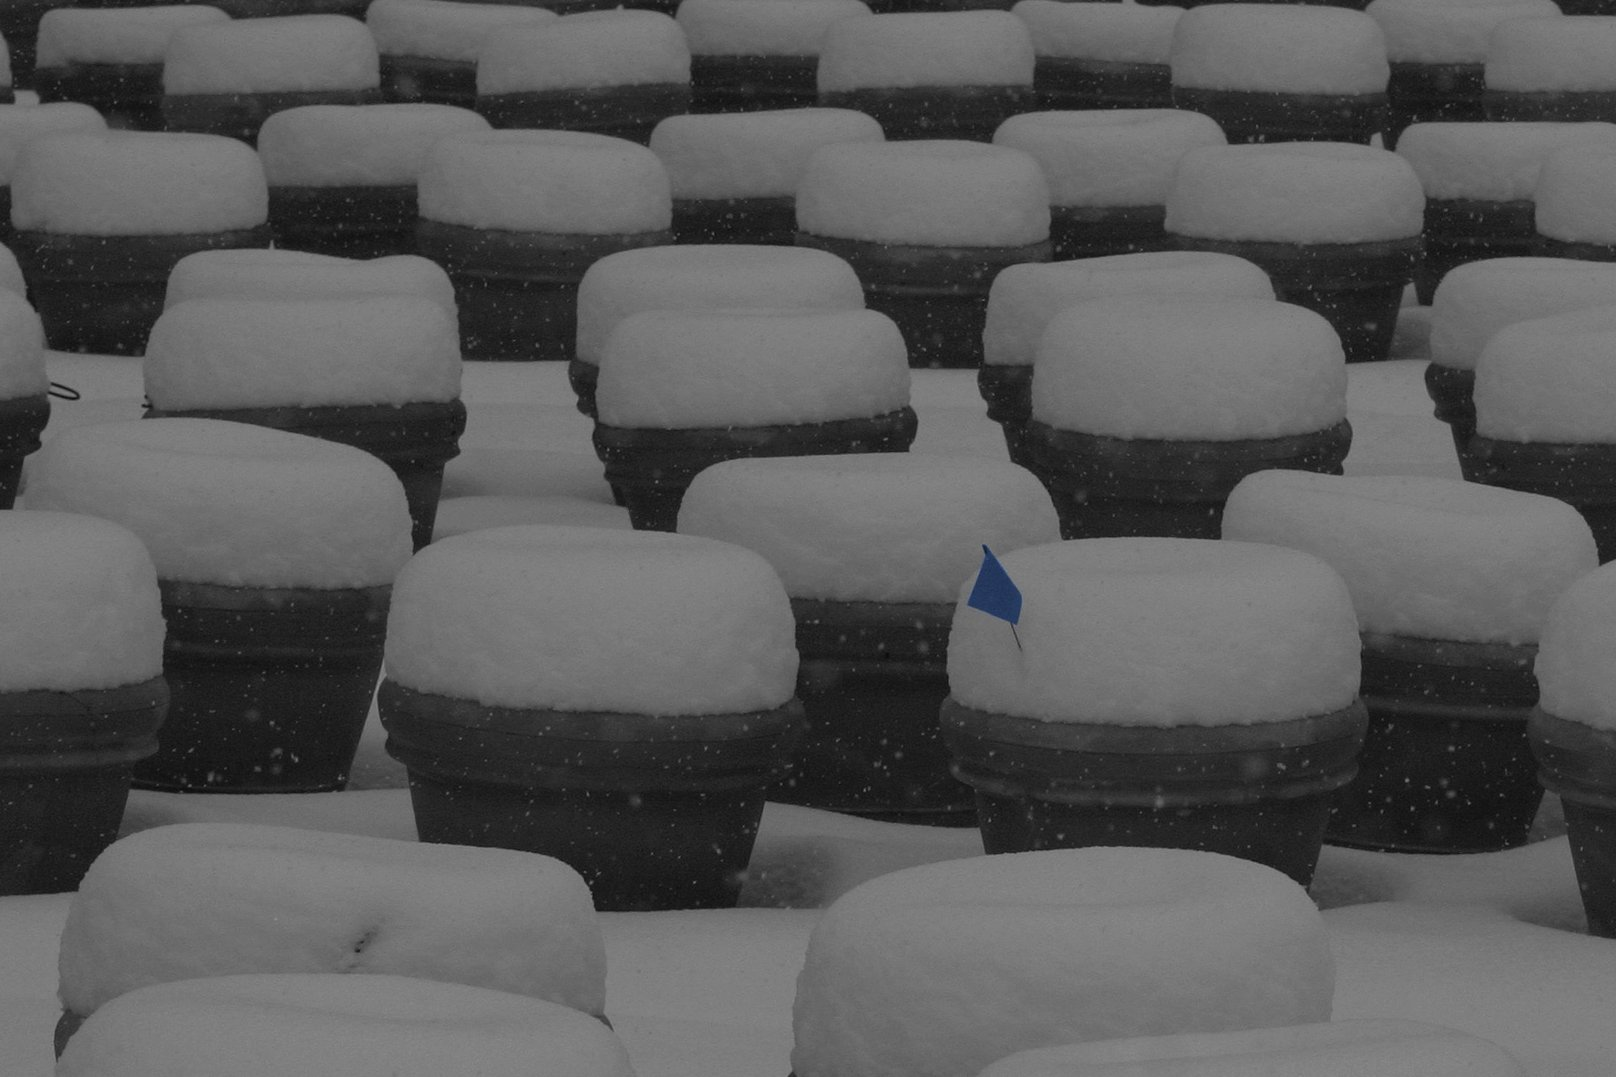
\includegraphics[width=7in]{../static/color/blue_flag.jpg}
\vfill
\newpage

\begin{paracol}{2}
\begin{leftcolumn}
July 3rd, 2004, shortly after midnight.

\begin{quotation}
Greens covering my chest and shoulders warmly are happiness.
\end{quotation}
\end{leftcolumn}
\end{paracol}

\begin{center}
\noindent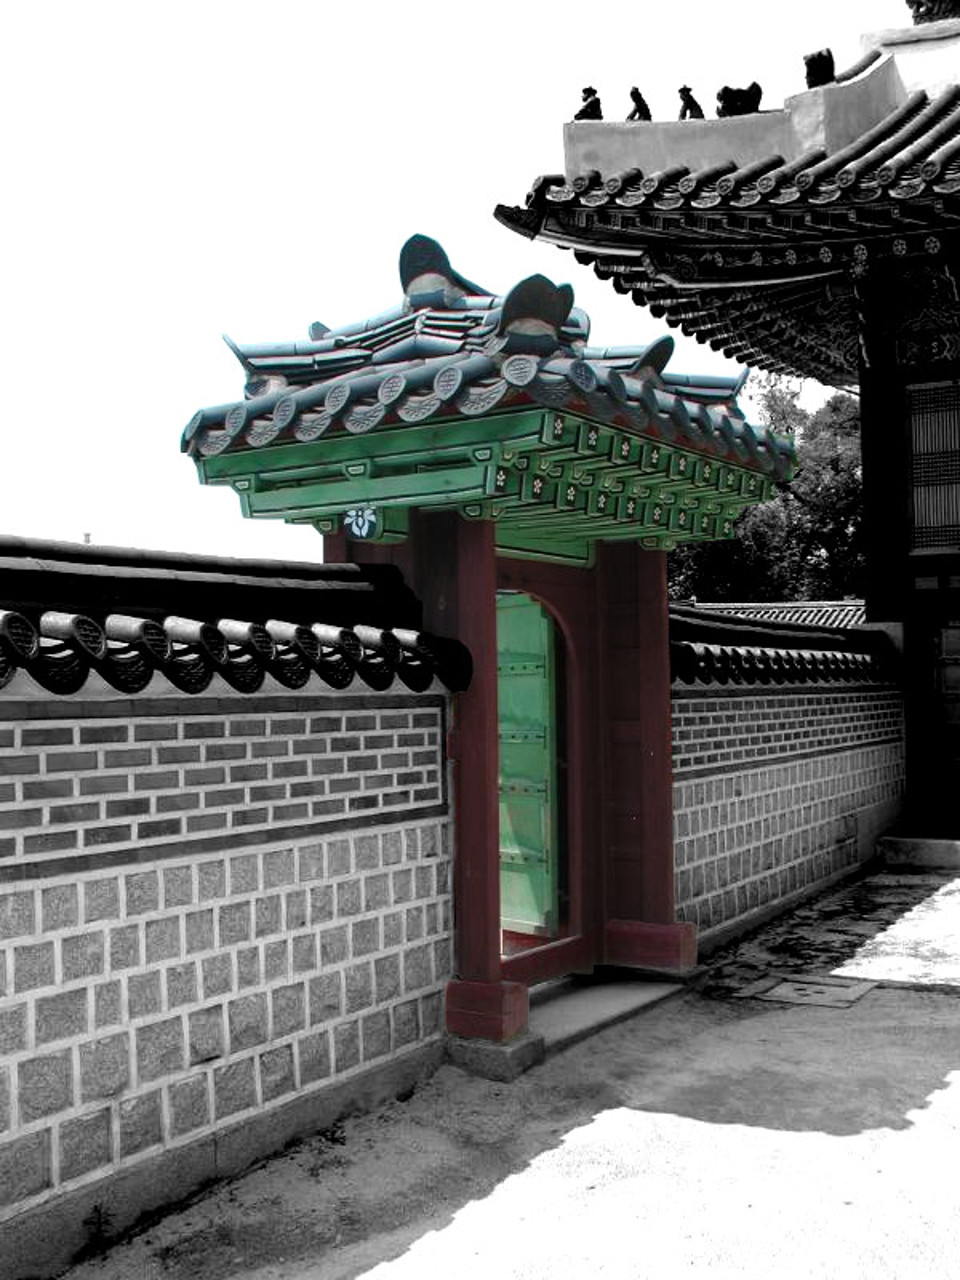
\includegraphics[width=4in]{../static/color/green_door.jpg}
\end{center}

\begin{paracol}{2}
\begin{leftcolumn}
\ally{And that's when I showed up, yes?}

Yeah, later that day.

\begin{quotation}
The navy blue I've been seeing at waist level in front of me and to my left is contentment.  I'm not entirely sure that it being omnipresent is a good thing, however, considering the colors it's mixed with.  Am I really content with longing and hopelessness?  It's not out of the question, I suppose that it could just be another aspect of my personality.  But that just brings up the question of whether or not it's something I ingrained into myself through habit, something where I just kinda accepted that feeling such things is normal, okay, and what I want; or is it something I was born with, or that we're all born with?  Is it a side effect of love, expecting impossible desires and the blind hopelessness that follows the end of a four year undertaking?

\ally{Whatever, you're rambling.}

Guilty, conspirator.
\end{quotation}

\ally{And these pictures?}

All from years later. The color thing comes and goes, like you.

April 8, 2004

\begin{verse}
The undersides\\
\vin \vin off gray\\
\vin of clouds\\
\vin drift\\
\vin \vin while I\\
\vin \vin \vin on the path\\
\vin \vin stand\\
\vin above\\
\vin \vin where the crow flies\\
\vin me.\\
Off\\
\vin \vin with purple\\
\vin gray, I\\
\vin \vin wandering\\
\vin ponder, should\\
\vin \vin in a perfect\\
\vin \vin \vin were there such a thing\\
\vin \vin world\\
\vin be a\\
\vin \vin though the word is plain\\
\vin color with it's own\\
\vin \vin to name\\
\vin \vin \vin as they say\\
\vin \vin creates\\
\vin word.\\
It soothes.
\end{verse}

Sometimes I'm overcome by the numinous. Sometimes it's colors, sometimes it's you, sometimes it's a silence swelling within my chest, stealing breath.

\ally{He would be riding on the subway or writing formulas on the blackboard or having a meal or (as now) sitting and talking to someone across a table, and it would envelop him like a soundless tsunami.}

That's a post-rock song title.

\ally{Is it wrong?}

\noindent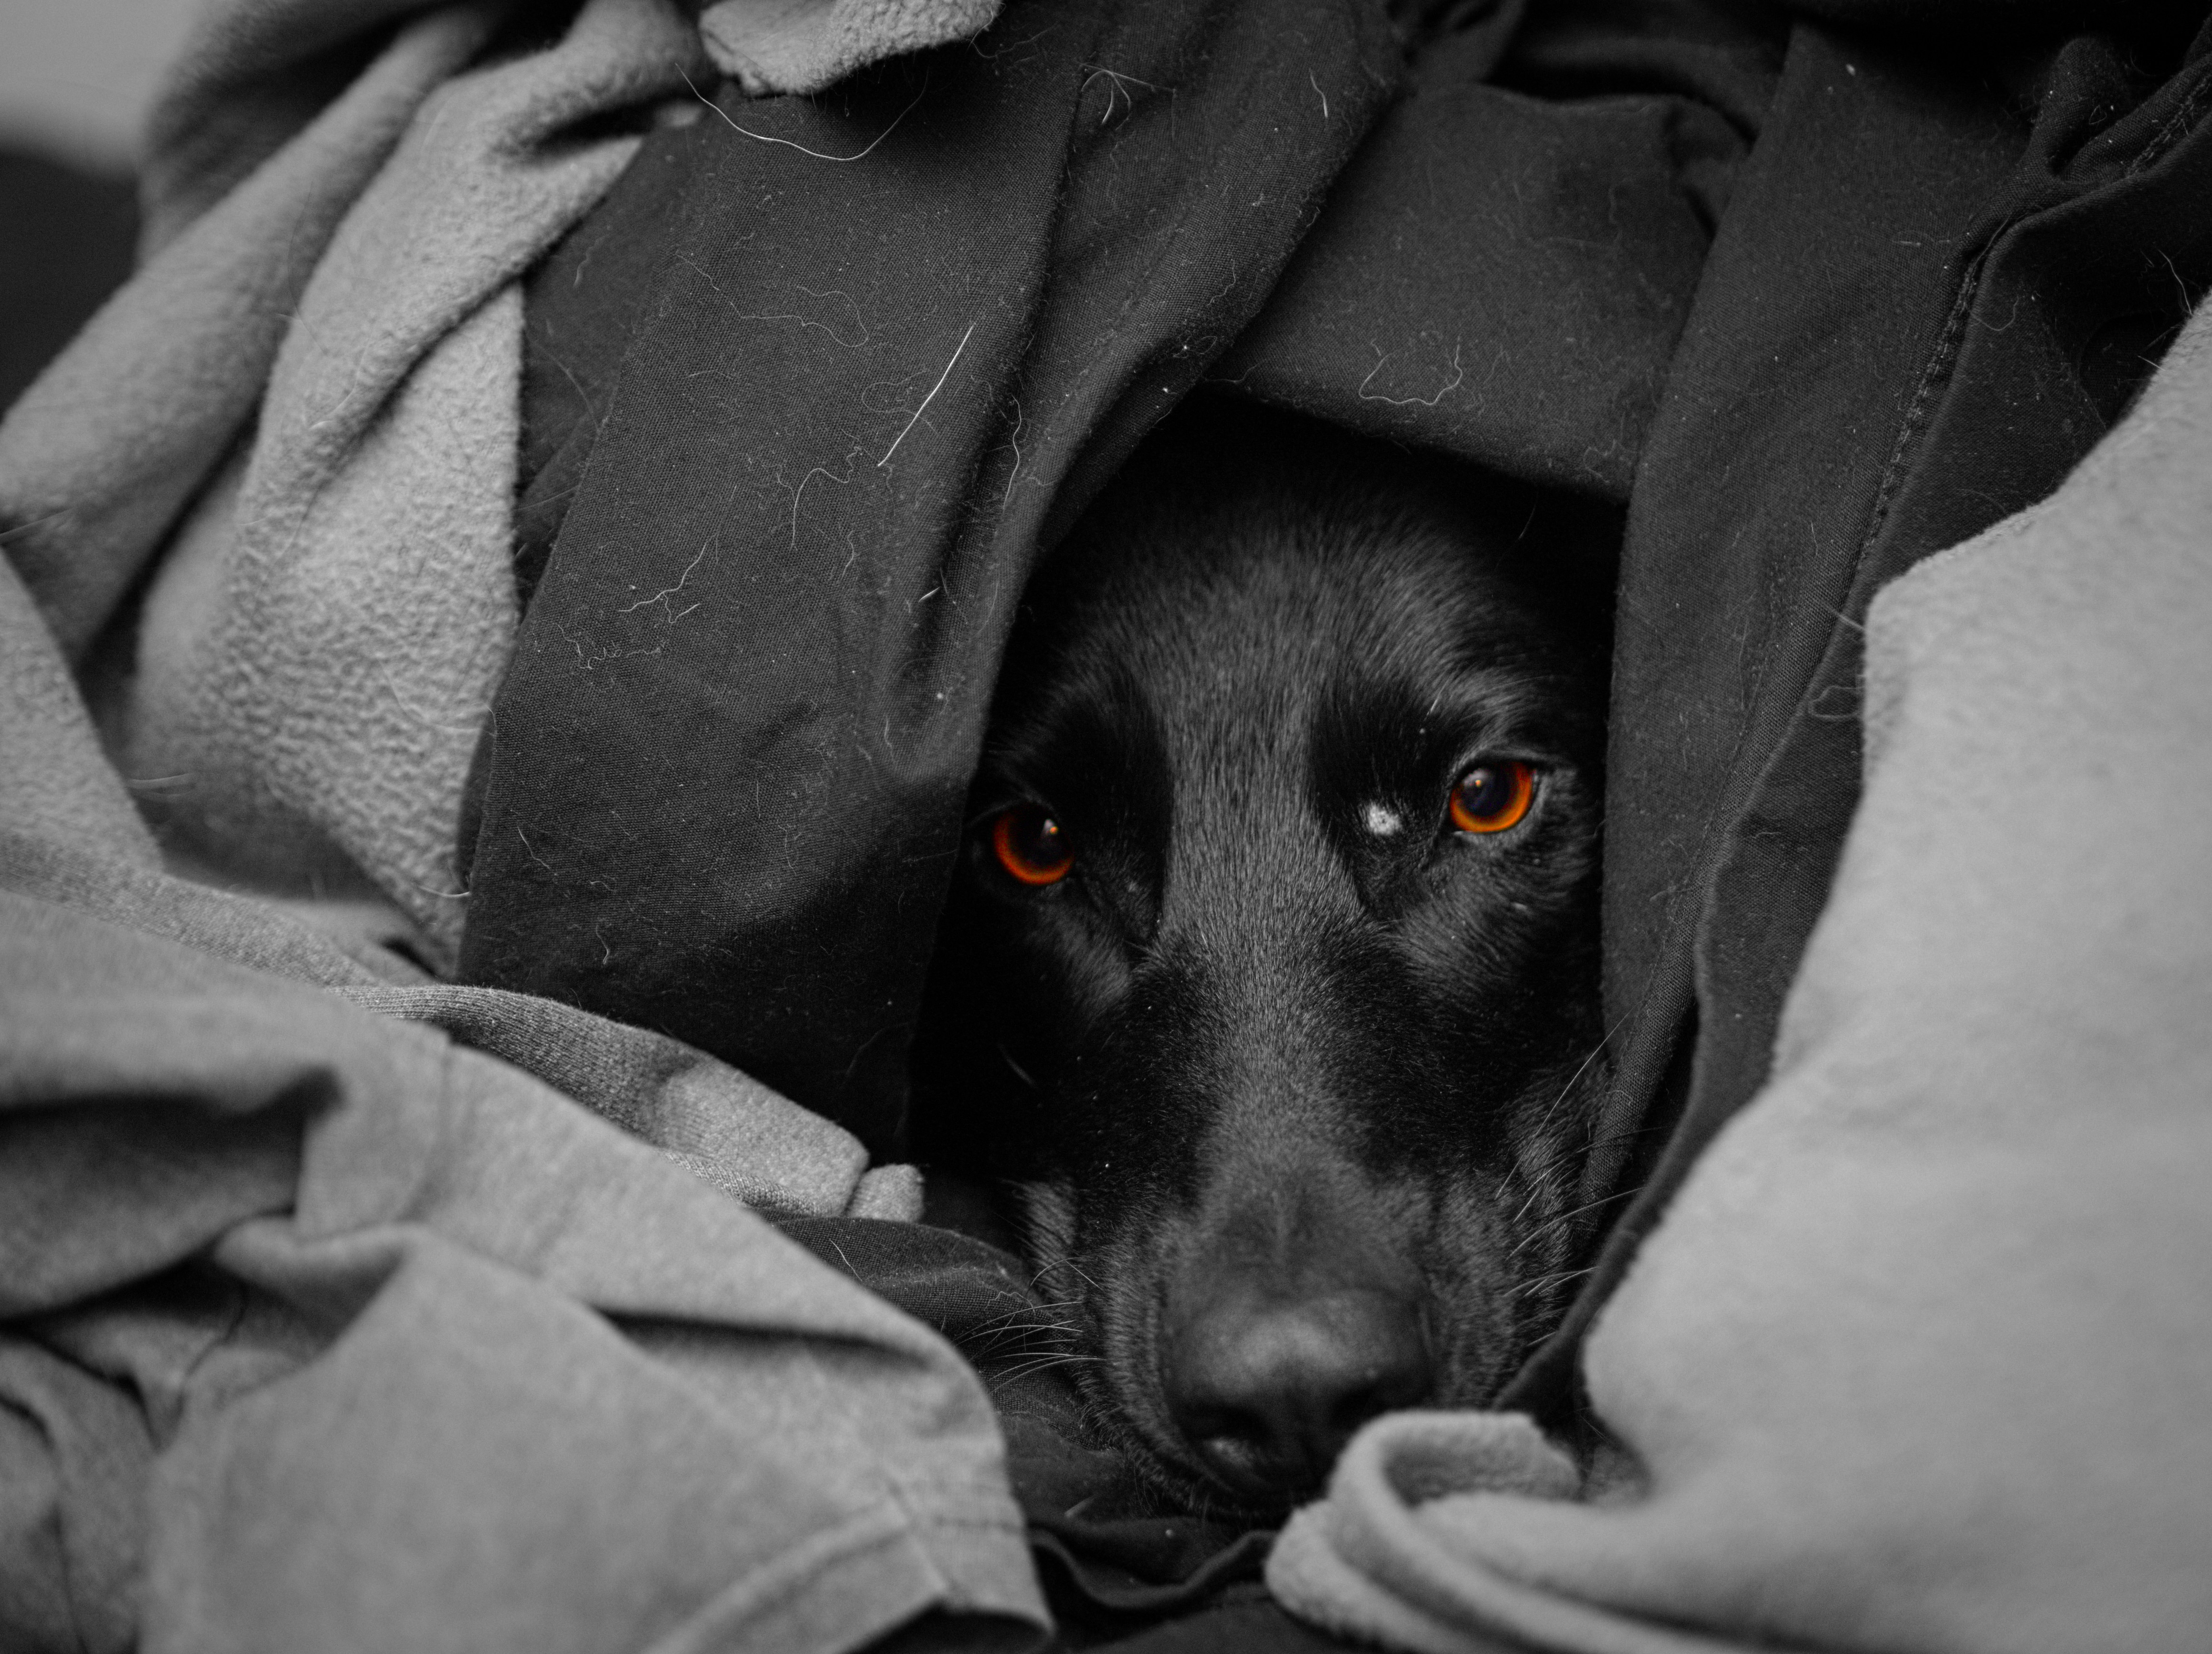
\includegraphics[width=4.35in]{../static/color/orange_eyes.jpg}

I'll take a picture, lasso a color, and desaturate everything else. Sometimes, it's fun. I do it to Falcon's eyes a lot because they're so pretty.

\ally{And sometimes it's something more.}

Yeah. Sometimes it's a compulsion. Sometimes a picture will latch onto me and never let me go. Sometimes I'll remove all color.


\noindent
\includegraphics[width=4.35in]{../static/color/bw1.jpg}

\noindent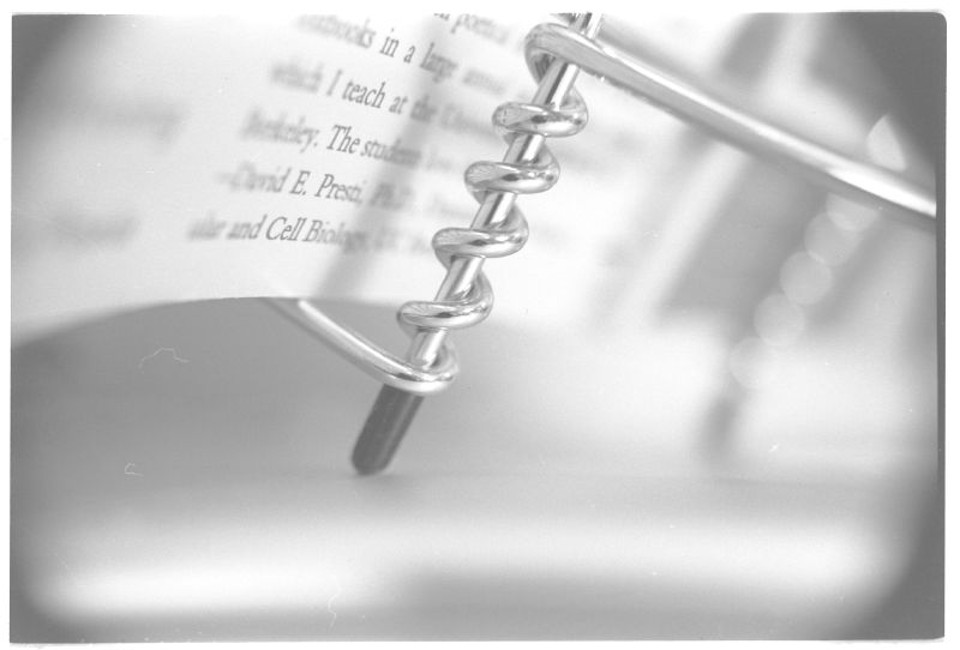
\includegraphics[width=4.35in]{../static/color/bw2.jpg}

\newpage

Sometimes I'll blow out the background because the foreground is so completely overwhelming.
\end{leftcolumn}
\end{paracol}
\vfill

\noindent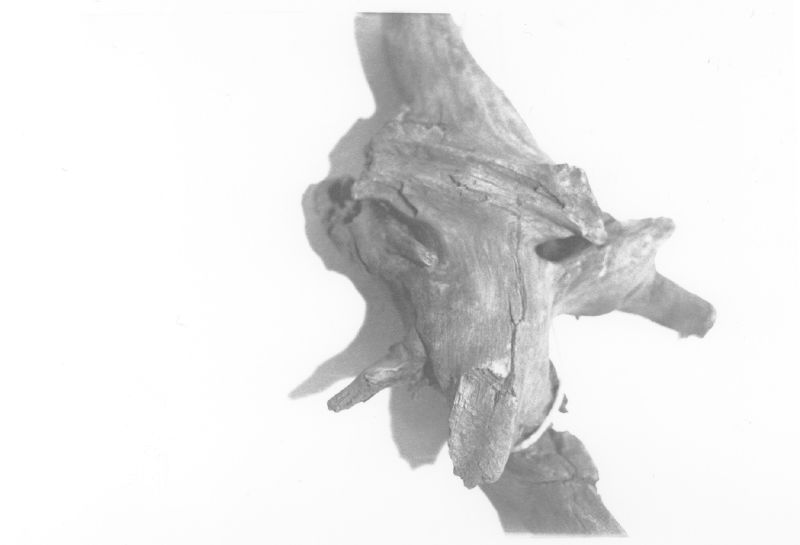
\includegraphics[width=7in]{../static/color/bw3.jpg}

\vfill
\newpage

Sometimes I'll skew colors all in one direction.
\vfill

\noindent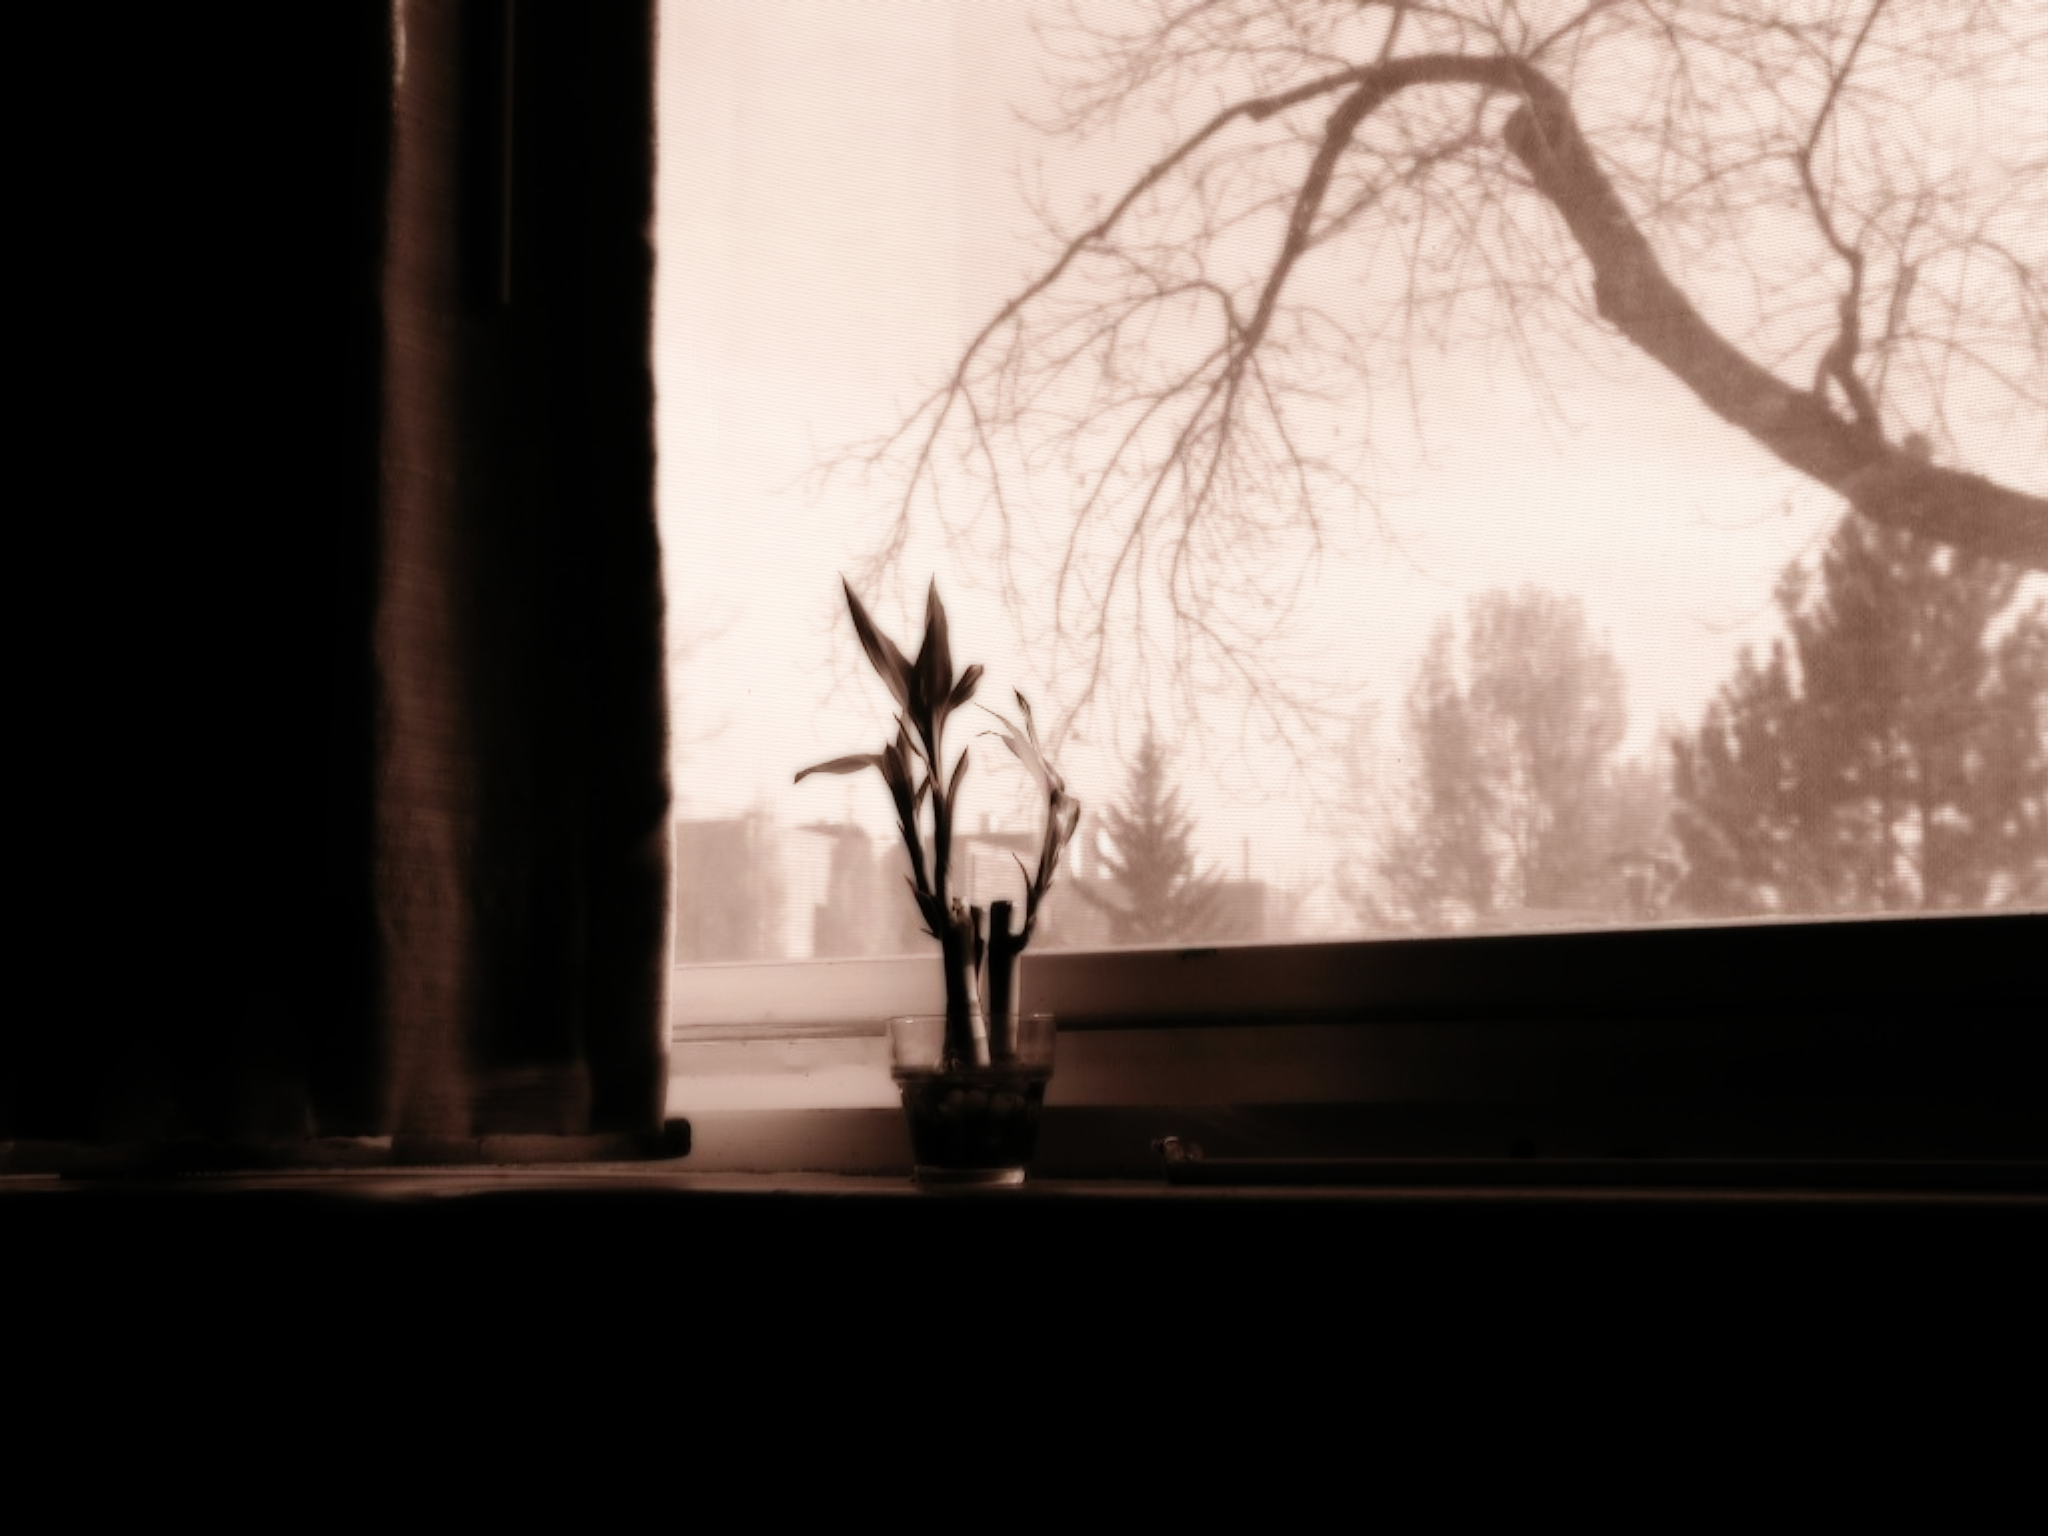
\includegraphics[width=7in]{../static/color/window_view.png}

\vfill
\newpage

\begin{paracol}{2}
\begin{rightcolumn}
    \null
    \vfill
    \noindent
\includegraphics[width=2.5in]{assets/3.png}

    \begin{quote}
    \emph{Lines and curves, lines and curves. Beginning now.}
    \end{quote}

    Seven o'clock, and the 13th Street crowd was headed to dinner, or focusing on a postprandial stroll.

    Jacob was focused on lines. On arcs and straight edges. On corners and angles.

    \begin{quote}
    \emph{The cans of spray-lubricant had clanked onto the counter, earlier that afternoon. Three of them, some of the cheap kind. The poor stoat behind the till scanned them numbly, seemingly on autopilot.}

    \emph{To see someone with such dead eyes had led down some strange alley and into what felt like second-hand embarrassment for Jacob. Second-hand to what, he couldn't tell. Either way, the transaction had itched, and he had shifted his weight from paw to paw until it was done.}

    \emph{Finally able to tap in the pin for his card, that itch had been scratched. The digits of the number across the pad always traced a pleasant, angular rune, and then the coyote was done, hurrying out of the store. The bag of cans had been dumped unceremoniously into one of the panniers of his bike, his tail clipped quickly to his thigh, and he had been off.}
    \end{quote}

    His breathing slowed and the jittery, speedy vibrations in his mind smoothed out.

    The heat along those lines grew, dull black iron turning first into a burgundy red, then glowing, picking up more towards cherry.

    \begin{quote}
    \emph{Spring turning to summer had the days warm, but not uncomfortably so. The air still held enough spring in it that the light long-sleeved shirt Jacob wore never got too warm, even with the exertion of the brisk ride home.}
    \end{quote}

    Eyes focused on surroundings briefly, hunting for a patch he knew had to be somewhere here. Wander north, magnetic attraction.

    \begin{quote}
    \emph{Ducking into the apartment had taken only seconds, enough for him to toss two of the purchased cans on a counter and another into a backpack, then back out into the evening air. Back onto his bike. Back on the road.}
    \end{quote}

    Cherry red and up to yellow, starting to put off enough glow that it crept into his vision, a light-leak in the camera of his eyes.

    \begin{quote}
    \emph{Making it to the 13th Street Plaza had taken longer than expected, but perhaps that was for the best. The flames would shine brighter in twilight.}
    \end{quote}

    North, north along Linden. North to cross the plaza. North to pass the fountain.

    \begin{quote}
    \emph{Jacob had parked his bike at a rack in front of one of the 12th street shops, locking it with care. Of his two prized possessions, the bike was the most practical, and the thought of losing it was something he would barely allow to register. He would be more than just upset, he'd be fucked. The commute to work would go from twenty minutes to more than an hour on the bus system, a fact he knew well from when it was too cold to ride. He'd saved up for three months to get this bike, a fantastic upgrade from what he'd had in college.}
    \end{quote}

    He could barely see now. Yellow brightened, headed more towards white. A sun made of lines, graceful arcs and definitive straightedges.

    \begin{quote}
    \emph{The other prized possession was less immediately practical, yet even more dear than the bike. The small sketchbook, barely more than a few inches on each side, was truly irreplaceable. That sat snugly in his pocket; the backpack was too risky, even his apartment wasn't safe enough.}
    \end{quote}

    Toward the courthouse.

    Jacob was panting now. Cool as the evening was getting, it was no match for the searing symbol locked in his thoughts. Burning, some part of him reddening, blistering, flaking and charring.

    \begin{quote}
    \emph{His Sigillarium sat distinct from his notes. Those were ash now, long gone. Their pages had held letters, all unique, warped and twisted through repeated passes of his pen, slipping and sliding together into some place between joy and fear, a place of too much meaning.}
    \end{quote}

    Past the courthouse now. And there, along the brick wall that surrounded the guarded parking lot. A place for moving the guilty to prison, maybe? There was the icy patch, freezing in the still-warm evening.

    \begin{quote}
    \emph{Once the meaning grew overwhelming---he'd know the moment when it came---the Sigillarium was brought out, opened reverently to the next blank page, and impressed with the new sigil. He used a dip pen with India ink into which he'd stirred several drops of blood. As the ink dried, Jacob did his best to start the process of forgetting.}
    \end{quote}

    Strange place, strange place. Empty, yet meaningful. Locked up. Guilty and innocent. Shackled, manacled, clanking and clinking in chains. The patch on the wall likely wasn't actually cold to the touch, yet he knew if he touched it, frostbite would follow.

    \begin{quote}
    \emph{Forgetting took days, weeks, months. It began with closing the Sigillarium, locking away intent and meaning while Jacob forgot the words themselves. He wouldn't look at the sigil again until the night before.}
    \end{quote}

    Obscured though his vision was, Jacob turned around, using his peripheral vision as best he could to check for others around.

    Empty street.

    \begin{quote}
    \emph{Doubtless there were cameras who had seen him, but intent never left a visible mark, so no one had ever come after him. Intent was psychological. Magical graffiti for no one to see and everyone to feel. He would begin internalizing the symbol the night before, and hold it in his mind until the moment of, when it once more became unbearable.}
    \end{quote}

    Smooth movements. Smooth and sure. He took the can, focused on the frigid patch, and began spraying. He couldn't do it too quickly, even if he did need to hurry. There needed to be enough penetrating oil left to burn.

    \begin{quote}
    \emph{Then he would bike and hunt for the cold he knew peppered the town.}
    \end{quote}

    The sigil was one unbroken line. One line that contained all those arcs and curves and straightaways and angles and corners. All sprayed dead center in the midst of that patch layering intent over what meaning was already there.

    Quickly, before he even capped the can, he fished his lighter out of his pocket and gave the wheel a rasp just at the final endpoint of the line.

    Blue flames, tinged yellow at the tips, spread fast, curling along the sigil, branching and curving whenever it came across a point where lines crossed.

    All that fire in his mind wound up on stone.

    All that patch of ice began to thaw.

    The coyote was already on his way back to the plaza, can of lubricant back in his bag and all that unbearable meaning seeping from him as he slipped into the evening crowd.

\end{rightcolumn}
\begin{leftcolumn}
It's not an artistic decision. Not \emph{just}, at least. It's always something more.

\begin{verse}
Inter ĝuo kaj timo\\
Estas loko de tro da signifo.\\
Apud kompreno, ekster saĝo,\\
Tamen ĝi tutampleksas.\\
Mi kompareble malgrandas\\
Kaj ĝi tro granda estas.\\
Nekomprenebla\\
Nekontestebla,\\
Senmova kaj ĉiam ŝanĝiĝema.

Between joy and fear\\
Is a place of too much meaning.\\
Next to understanding, outside wisdom,\\
It nonetheless expands.\\
I'm so small beside it\\
and it is too big.\\
Incomprehensible,\\
Incontestible,\\
Unmoving and always changing.
\end{verse}

A sigil need not just be lines and curves.

\ally{Or maybe it's just mania.}

It may be.
